\begin{figure}[htbp]
\centering
\definecolor{moduleink}{RGB}{40,82,94}
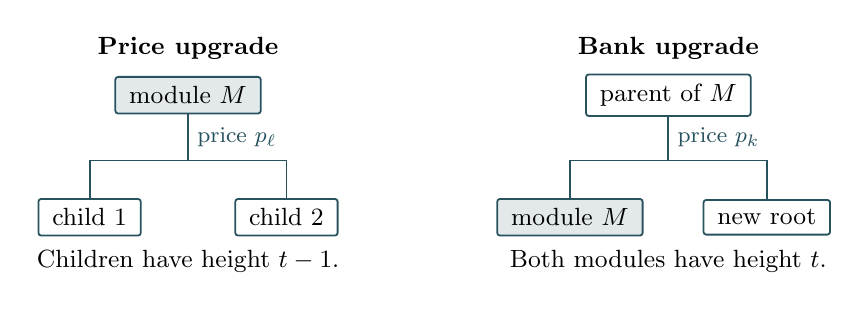
\begin{tikzpicture}[x=1cm,y=1cm,font=\small,line width=.65pt,
  module/.style={draw=moduleink,rounded corners=1pt,inner xsep=5pt,inner ysep=3.5pt},
  current/.style={module,fill=moduleink!13},edge/.style={draw=moduleink},
  linklabel/.style={font=\footnotesize,text=moduleink,fill=white,inner sep=1.3pt}]
  \node at (0,2.15) {\textbf{Price upgrade}};
  \node[current] (m) at (0,1.55) {module \(M\)};
  \node[module] (c1) at (-1.25,0) {child \(1\)};
  \node[module] (c2) at (1.25,0) {child \(2\)};
  \draw[edge] (m.south) -- (0,.72) -- (-1.25,.72) -- (c1.north);
  \draw[edge] (0,.72) -- (1.25,.72) -- (c2.north);
  \node[linklabel,anchor=west] at (.06,1.02) {price \(p_\ell\)};
  \node at (0,-.56) {Children have height \(t-1\).};
  \begin{scope}[shift={(6.1,0)}]
    \node at (0,2.15) {\textbf{Bank upgrade}};
    \node[module] (up) at (0,1.55) {parent of \(M\)};
    \node[current] (old) at (-1.25,0) {module \(M\)};
    \node[module] (new) at (1.25,0) {new root};
    \draw[edge] (up.south) -- (0,.72) -- (-1.25,.72) -- (old.north);
    \draw[edge] (0,.72) -- (1.25,.72) -- (new.north);
    \node[linklabel,anchor=west] at (.06,1.02) {price \(p_k\)};
    \node at (0,-.56) {Both modules have height \(t\).};
  \end{scope}
\end{tikzpicture}
\caption{The two physical attachments for an upgrade at module \(M\) of
height \(t\). At a price upgrade, child outputs \(v_1,v_2\) reach \(M\)
as \(p_\ell+\varepsilon v_1\) and \(p_\ell+\varepsilon v_2\).
A bank upgrade places its new roots alongside \(M\), at the same incoming
price \(p_k\) when \(M\) has a parent.}
\label{fig:request-upgrades}
\end{figure}
